% 真实照片取自开放获取论文；非本团队拍摄，非本模型实测验证。
% 完整出处、原出版PDF与SHA256见review/photo_sources.json及review/photo_archive。
图\ref{fig:real-site-context}引用新疆大学研究人员在乌鲁木齐开展既有建筑改造研究时的建筑与热流计实拍\supcite{33}。

\begin{figure}[htbp]
\centering
\begin{minipage}[t]{0.44\textwidth}
\centering
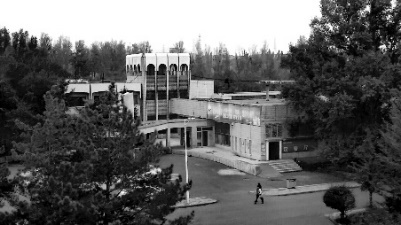
\includegraphics[height=34mm,width=\linewidth,keepaspectratio]{media/site_photos/urumqi_hotel_building.png}
\par\small （a）乌鲁木齐南郊既有旅馆
\end{minipage}\hfill
\begin{minipage}[t]{0.44\textwidth}
\centering
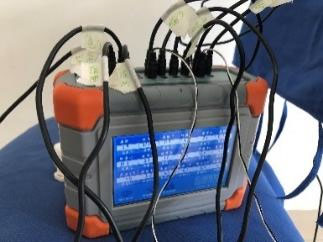
\includegraphics[height=34mm,width=\linewidth,keepaspectratio]{media/site_photos/urumqi_hotel_heat_flux_measurement.jpeg}
\par\small （b）现场使用的多通道热流计
\end{minipage}
\caption{乌鲁木齐既有建筑与热流测量现场。取自Liao等\supcite{33}原图1左、图5左，CC BY 4.0；等比例排版，未修改照片内容。}
\label{fig:real-site-context}
\end{figure}
